%%% template.annotated.tex
%%%
%%% This LaTeX source document can be used as the basis for your technical
%%% paper or abstract. Unlike ``template.tex,'' this version of the source
%%% document contains documentation of each of the commands and definitions
%%% that should be used in the preparation of your formatted document.
%%% 
%%% The parameter given to the ``acmsiggraph'' LaTeX class in the 
%%% ``\documentclass'' command controls several features of the formatted 
%%% output: the presence or absence of hyperlinked icons just prior to the 
%%% first section of the paper, the amount of space left clear for the ACM
%%% copyright notice, the presence or absence of line numbers and submission
%%% ID, and the presence or absence of an appropriate ``preprint'' notice.
%%% 
%%% If you are preparing a paper for presentation in the Technical Papers
%%% program at one of our two annual flagship conferences, held in North 
%%% America (SIGGRAPH) or Asia (SIGGRAPH Asia), you should use ``tog''
%%% as the parameter.
%%%
%%% If you are preparing a paper for presentation at one of our sponsored
%%% events, including SIGGRAPH and SIGGRAPH Asia, but not in those events' 
%%% Technical Papers program, or a one- to four-page abstract, you should 
%%% use ``conference'' as the parameter.
%%% (Technical Briefs and Game Papers presented at our annual flagship 
%%% events fall into this category, as do papers accepted to other SIGGRAPH-
%%% sponsored events, such as I3D or ETRA or VRCAI, as do the one-page 
%%% abstracts which serve as the primary documentation for many of our 
%%% annual conference programs, including Posters, Talks, and Emerging 
%%% Technologies.)
%%%
%%% If you are preparing a version of your content for review, you should
%%% use ``review'' as the parameter. Line numbers will be added to your 
%%% paper, and the submission ID value will be printed across the top of 
%%% each page of your paper. (Use the submission ID as the parameter to the
%%% ``TOGonlineID'' command, below.)
%%%
%%% If you are preparing a preprint of your content, you should use
%%% ``preprint'' as the parameter. This is primarily for annual conference
%%% papers; a header reading ``To appear in ACM TOG X(Y)'' will appear on
%%% each page of the formatted output (where X is the volume and Y is the 
%%% number of the issue in which it will be published).

\documentclass[tog]{acmsiggraph}

%%% Definitions and commands that begin with ``\TOG'' are meant to be used
%%% in the preparation of papers to be presented in the Technical Papers
%%% program at one of our annual flagship events - SIGGRAPH and SIGGRAPH 
%%% Asia. You can safely ignore these definitions and commands if your 
%%% content is to be presented in some other venue.

%%% ``\TOGonlineid'' should be filled with the online ID value you received
%%% when you submitted your technical paper. It will be printed out if you 
%%% prepare a ``review'' version of your paper.

\TOGonlineid{45678}

%%% Should your technical paper be accepted, you will be given three pieces
%%% of information: the volume and number of the issue of the ACM Transactions
%%% on Graphics journal in which your paper will be published, and the 
%%% ``article DOI'' value, which is unique to your paper and provides the 
%%% link to your paper's page in the ACM Digital Library. Fill in the 
%%% ``\TOGvolume,'' ``\TOGnumber,'' and ``\TOGarticleDOI'' definitions with
%%% the three pieces of information you receive.

\TOGvolume{0}
\TOGnumber{0}
\TOGarticleDOI{1111111.2222222}

%%% By default, your technical paper will contain hyperlinked icons which 
%%% point to your paper's article page in the ACM Digital Library, and to 
%%% the paper itself in the ACM Digital Library. You may wish to add one 
%%% or more links to your own resources. If any of the following four 
%%% definitions have URLs in them, an appropriate hyperlinked icon will be
%%% added to the list. 

\TOGprojectURL{}
\TOGvideoURL{}
\TOGdataURL{}
\TOGcodeURL{}

%%% Define the title of your paper here. Use capital letters as appropriate.
%%% Setting the entire title in upper-case letters is not correct, nor is 
%%% capitalizing only the first letter of the title.

\title{Project Proposal for Physically Based Animation: Fracture
  Simulation in Two and Three Dimensions}

%%% Define the author list in the ``\author'' command. The ``\thanks'' 
%%% field can be used to define an e-mail address for the author.
%%% The ``\pdfauthor'' field should contain a comma-separated list of the
%%% authors of the paper, and is used, along with the title and keyword
%%% data, for PDF metadata. (To see this metadata, open the PDF in Adobe 
%%% Reader and select ``File > Properties > Description.''

\author{Ari Karo, Chris
  Yu\thanks{e-mail:\{aak82,cy284\}@cornell.edu}\\Cornell University}
\pdfauthor{Robert A. Smith}

%%% User-defined keywords.

\keywords{cs5643, final project, proposal, fracture simulation}

%%% End of the document preamble, start of the document.

\begin{document}

%%% A ``teaser'' image appears below the title and affiliation and above
%%% the two-column body of the paper. This is optional, but if you wish
%%% to include such an image, the commented-out code, below, can be used
%%% as an example. Please note that the inclusion of a ``teaser'' image
%%% may move the copyright space to the bottom of the right-hand column
%%% on the first page of your formatted output. This is acceptable.

 \teaser{
   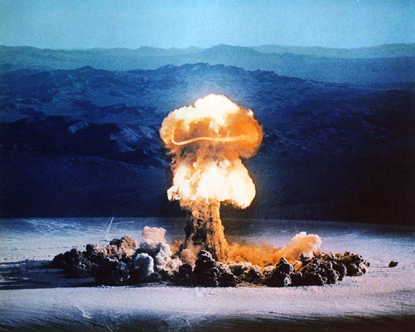
\includegraphics[height=1.5in]{images/explode.jpg}
   \caption{An example of a scenario that may call for fracturing objects.}
}

%%% The ``\maketitle'' command uses the author and title information 
%%% defined above, and prepares the formatted title.

\maketitle

%%% The ``abstract'' environment should contain the abstract for your
%%% content -- one to several paragraphs which describe the work.

\begin{abstract}

Here, we propose a project focused on the implementation of dynamic
fracture simulations, as detailed in \cite{Mul13}. The method
described is an improvement on previous methods for fracture
simulations, which typically involve using pre-fractured models and
replacing objects with these fragments at runtime. These older methods
have the disadvantage that fracture patterns generally do not match
the impact location. The newer method uses volumetric approximate
convex decompositions (VACDs), whereby pre-defined fracture patterns
are applied to the pieces of geometry, and the geometry is
subsequently split into a non-overlapping convex cover of itself.  The
method described in \cite{Mul13} is quite detailed, and we plan to
first handle the simpler task of implementing it in two dimensions,
before possibly adapting our implementation (time-permitting) to three
dimensions.

\end{abstract}

%%% The ``CRCatlist'' environment defines one or more ACM ``Computing Review''
%%% (or ``CR'') categories, used for indexing your work. For more information
%%% on CR categories, please see http://www.acm.org/class/1998.

\begin{CRcatlist}
  \CRcat{5643}{Computer Graphics}{Physically Based Animation}{Fracturing}
\end{CRcatlist}

%%% The ``\keywordlist'' prints out the user-defined keywords.

\keywordlist

%%% If you are preparing a paper to be presented in the Technical Papers
%%% program at one of our annual flagship events (and, therefore, using 
%%% the ``tog'' parameter to the ``\documentclass'' command), the 
%%% ``\TOGlinkslist'' command prints out the list of hyperlinked icons.
%%% If you are using any other parameter to the ``\documentclass'' command
%%% this command does absolutely nothing.

%\TOGlinkslist

%%% The ``\copyrightspace'' command will leave clear an amount of space
%%% at the bottom of the left-hand column on the first page of your paper,
%%% according to the parameter used in the ``\documentclass'' command.

\copyrightspace

%%% The first section of your paper. 

\section{Introduction}

Simulations of fracturing objects are becoming increasingly applicable
and desirable in media such as movies and games, where, depending on
the genre, scenes of massive and wanton destruction may be
commonplace. Particularly in the context of video games, the prospect
of every rigid object being indestructible may be perceived as
implausible by an observer. While pre-fracturing is an option for
interactive simulations, this requires additional work for every
breakable asset, and prevents the pattern of fracture from depending
on the point of impact. There are also various other drawbacks, such
as pieces of objects being unable to break further without
preemptively preparing multiple levels of pre-fracturing.

A dynamic fracture simulation could potentially save time in producing
these assets, in addition to providing additional realism by allowing
objects to fracture in different ways, depending on the direction and
location of impact. In \cite{Mul13}, M\"uller et al. present a new
method for such dynamic fractures, which simultaneously preserves
interactive speeds.

\section{Related Work}

The primary paper we will be focusing on is M\"uller et
al. \cite{Mul13} where the methods and algorithms for dynamic fracture
simulation are presented. Before this paper, various other methods for
fracture simulation had been described, dating back as early as
Terzopoulos et al. \cite{Ter88} and Norton et al. \cite{Nor91}, the
latter making use of a mass-spring model. O'Brien et al. \cite{Obr99}
presented a method that used continuum mechanics to compute internal
stresses and fracture directions.

Parker et al. \cite{Par09} proposed a method for fracture simulation
that used a relatively coarse tetrahedral mesh, where objects can
fracture only along the bounaries of the tetrahedra; in order to hide
the coarseness of the mesh, they also introduce ``splinters''
associated with each element. This method is primarily targeted at
computer games, as it runs at interactive speeds.

Pre-fracturing objects is a commonly-used approach in movies and
games, as mentioned, and a wide array of methods for breaking up
objects has been proposed. A few of the many techniques include manual
cutting by artists, image guidance \cite{Mou05}, Voronoi fracturing of
surfaces \cite{Rag02}, and tetrahedralization \cite{Par09}.

\section{Technical Description}

The method described only works with meshes that satisfy the following
three properties: (1) the meshes are composed of convex pieces, (2)
the pieces do not overlap, and (3) any two pieces are physically
connected if and only if the first piece has at least one face that
partially or fully overlaps one face of the second piece, and the two
faces are coplanar with opposite normals. A mesh satisfying this is
called a compound. Note that meshes created by volumetric approximate
convex decomposition satisfy this property by default; the exact
algorithm for performing the VACD is given in the paper.

The method uses fracture patterns, which are partitions of the entire
space into convex pieces. Once fracturing is called for, the following
steps are performed. The fracture pattern is first translated to align
with the impact location. We then compute all intersections of all
cells of the fracture pattern with all convex pieces of the
object. Next, in order to save computation time, we find all pieces
that are completely covered with newly created convexes, and replace
these all with a single convex with the same shape. All convexes
within the same cell are then combined to form a new
compound. Finally, we check for disconnected ``islands'' of convexes
that have been grouped into the same mesh, and turn them into separate
compounds.

\section{Proposal and Expectations}

What we plan to do.

\section{Extensions, time-permitting}

What we would like to do but aren't sure if we will have time for.

%%% Please use the ``acmsiggraph'' BibTeX style to properly format your
%%% bibliography.

\bibliographystyle{acmsiggraph}
\bibliography{template}

\end{document}
